\documentclass[10pt, UKenglish]{beamer}
\usepackage{babel}
\usepackage[utf8]{inputenc}  
\usepackage{geometry}
\usepackage[customcolors]{hf-tikz}
\usepackage[T1]{fontenc}   
\usepackage{tcolorbox}
\usepackage{siunitx}
\usepackage{hyperref}
\usepackage{bookmark}
\usepackage{marvosym}
\usepackage{tikz}
\usepackage{tikz-qtree}
\usepackage{cancel}
\usepackage{todonotes}
\useoutertheme[subsection=false]{smoothbars}
\DeclareSIUnit[number-unit-product = {}]{\inchQ}{\textquotedbl}
\usepackage{amsmath,bm}
\DeclareSIUnit[number-unit-product = {\thinspace}]{\inch}{in}
\usetheme[menuwidth={0.3\paperwidth}]{erlangen}
\usepackage{multicol}
\usepackage{charter}
\setbeamercovered{transparent=20}
\setbeamertemplate{navigation symbols}{}
\sisetup{separate-uncertainty = true}
\usepackage[version=4]{mhchem}
\usepackage{tikz}
\usepackage{hepnames}
\usepackage{soul}
\usepackage{color}
\usepackage{thesis_defs}
\usepackage{subcaption}
\captionsetup[subfigure]{labelformat=empty}
\usepackage{xcolor}


\usepackage[backend=biber]{biblatex}
\bibliography{bibliography.bib}

\graphicspath{%
  {./feynman_diagrams/}%
  {./figures_theory/}%
  {./figures_simple/}%
  {./figures_misc/}%
  {./app1/}%
  {./app2/}%
  {./misc/}%
  {./ANN_plots/} %
  {./NN_plots/} %
  {tagging_plots/}%
}


\definecolor{color1}{RGB}{33,217,217}
\definecolor{color2}{RGB}{7,61,111}

\newcommand{\lr}{\mathcal{lr}}


\newcounter{totavalue}
\newcounter{parvalue}

\def\aux{1}
\def\radius{9pt}
\def\step{4pt}
\usepackage[absolute,overlay]{textpos}


\newcommand\circcounter{%
\ifnum\inserttotalframenumber<2\relax
\else
  \setcounter{totavalue}{\inserttotalframenumber}
  \setcounter{parvalue}{\insertframenumber}
  \ifnum\inserttotalframenumber>45\relax
    \renewcommand\step{0pt}
  \fi%
  \pgfmathsetmacro{\aux}{360/35}
  \begin{tikzpicture}[remember picture,overlay, rotate=90+\aux]
  \foreach \i in {0,1,...,35}
    \fill[logo_blue] 
      (0,0) -- (-\i*\aux:\radius) arc  (-\i*\aux:-(\i+1)*\aux+\step:\radius) -- cycle;
  \foreach \i in {1,...,\insertframenumber}
    \fill[logo_grey] 
      (0,0) -- (-\i*\aux:\radius) arc  (-\i*\aux:-(\i+1)*\aux+\step:\radius) -- cycle;
  \fill[white] circle (\radius/1.3);
  \node at (0,0) {\small\insertframenumber}; 
  \end{tikzpicture}%
\fi%
}


\usepackage{eso-pic,picture}



\begin{document} 

\title[Bachelorvortrag]{Reducing the effect of nominal background samples on signal sample systematics using an adversarial neural network in the \tW dilepton channel}
\subtitle{18th of September 2019}
\author{Christian Kirfel}
%\institute{Universtität Bonn}
        



\begin{frame}[plain]
\vspace{0.0cm}
  \titlepage
      \AddToShipoutPictureFG*{%
    \AtPageUpperLeft{%
      \put(8.7cm,-9.6cm){

\includegraphics[scale=0.03]{original_logo.jpg}
\makebox(0,0)[lt]{}%
      }%
    }%
  }%
    \AddToShipoutPictureFG*{%
    \AtPageUpperLeft{%
      \put(0.0cm,-9.6cm){
%
\includegraphics[scale=0.17]{atlas_gay.png}

\includegraphics[scale=0.17]{ATLAS-Logo-Ref-RGB-H_0.jpg}
\makebox(0,0)[lt]{}%
      }%
    }%
  }%
\end{frame}
\addtobeamertemplate{navigation symbols}{\vspace*{0.8cm}\hfill\circcounter\hspace*{0.7cm}}

\section{Intro}

\begin{frame}{Outline}
\begin{itemize}
    \item $\Ptop\PW$ and $\Ptop\APtop$ separation
    \vspace{0.3cm}
    \item Artificial neural networks and adversarial neural networks as a possible solution
    \vspace{0.3cm}
    \item Introduction to hyperparameters
    \vspace{0.3cm}
    \item Preliminary training results for an adversarial neural network
\end{itemize}
\end{frame}

\begin{frame}{$\Ptop\PW$ and $\Ptop\APtop$ separation}
    \begin{columns}
    \begin{column}{0.5\textwidth}
        \begin{figure}
            \centering
            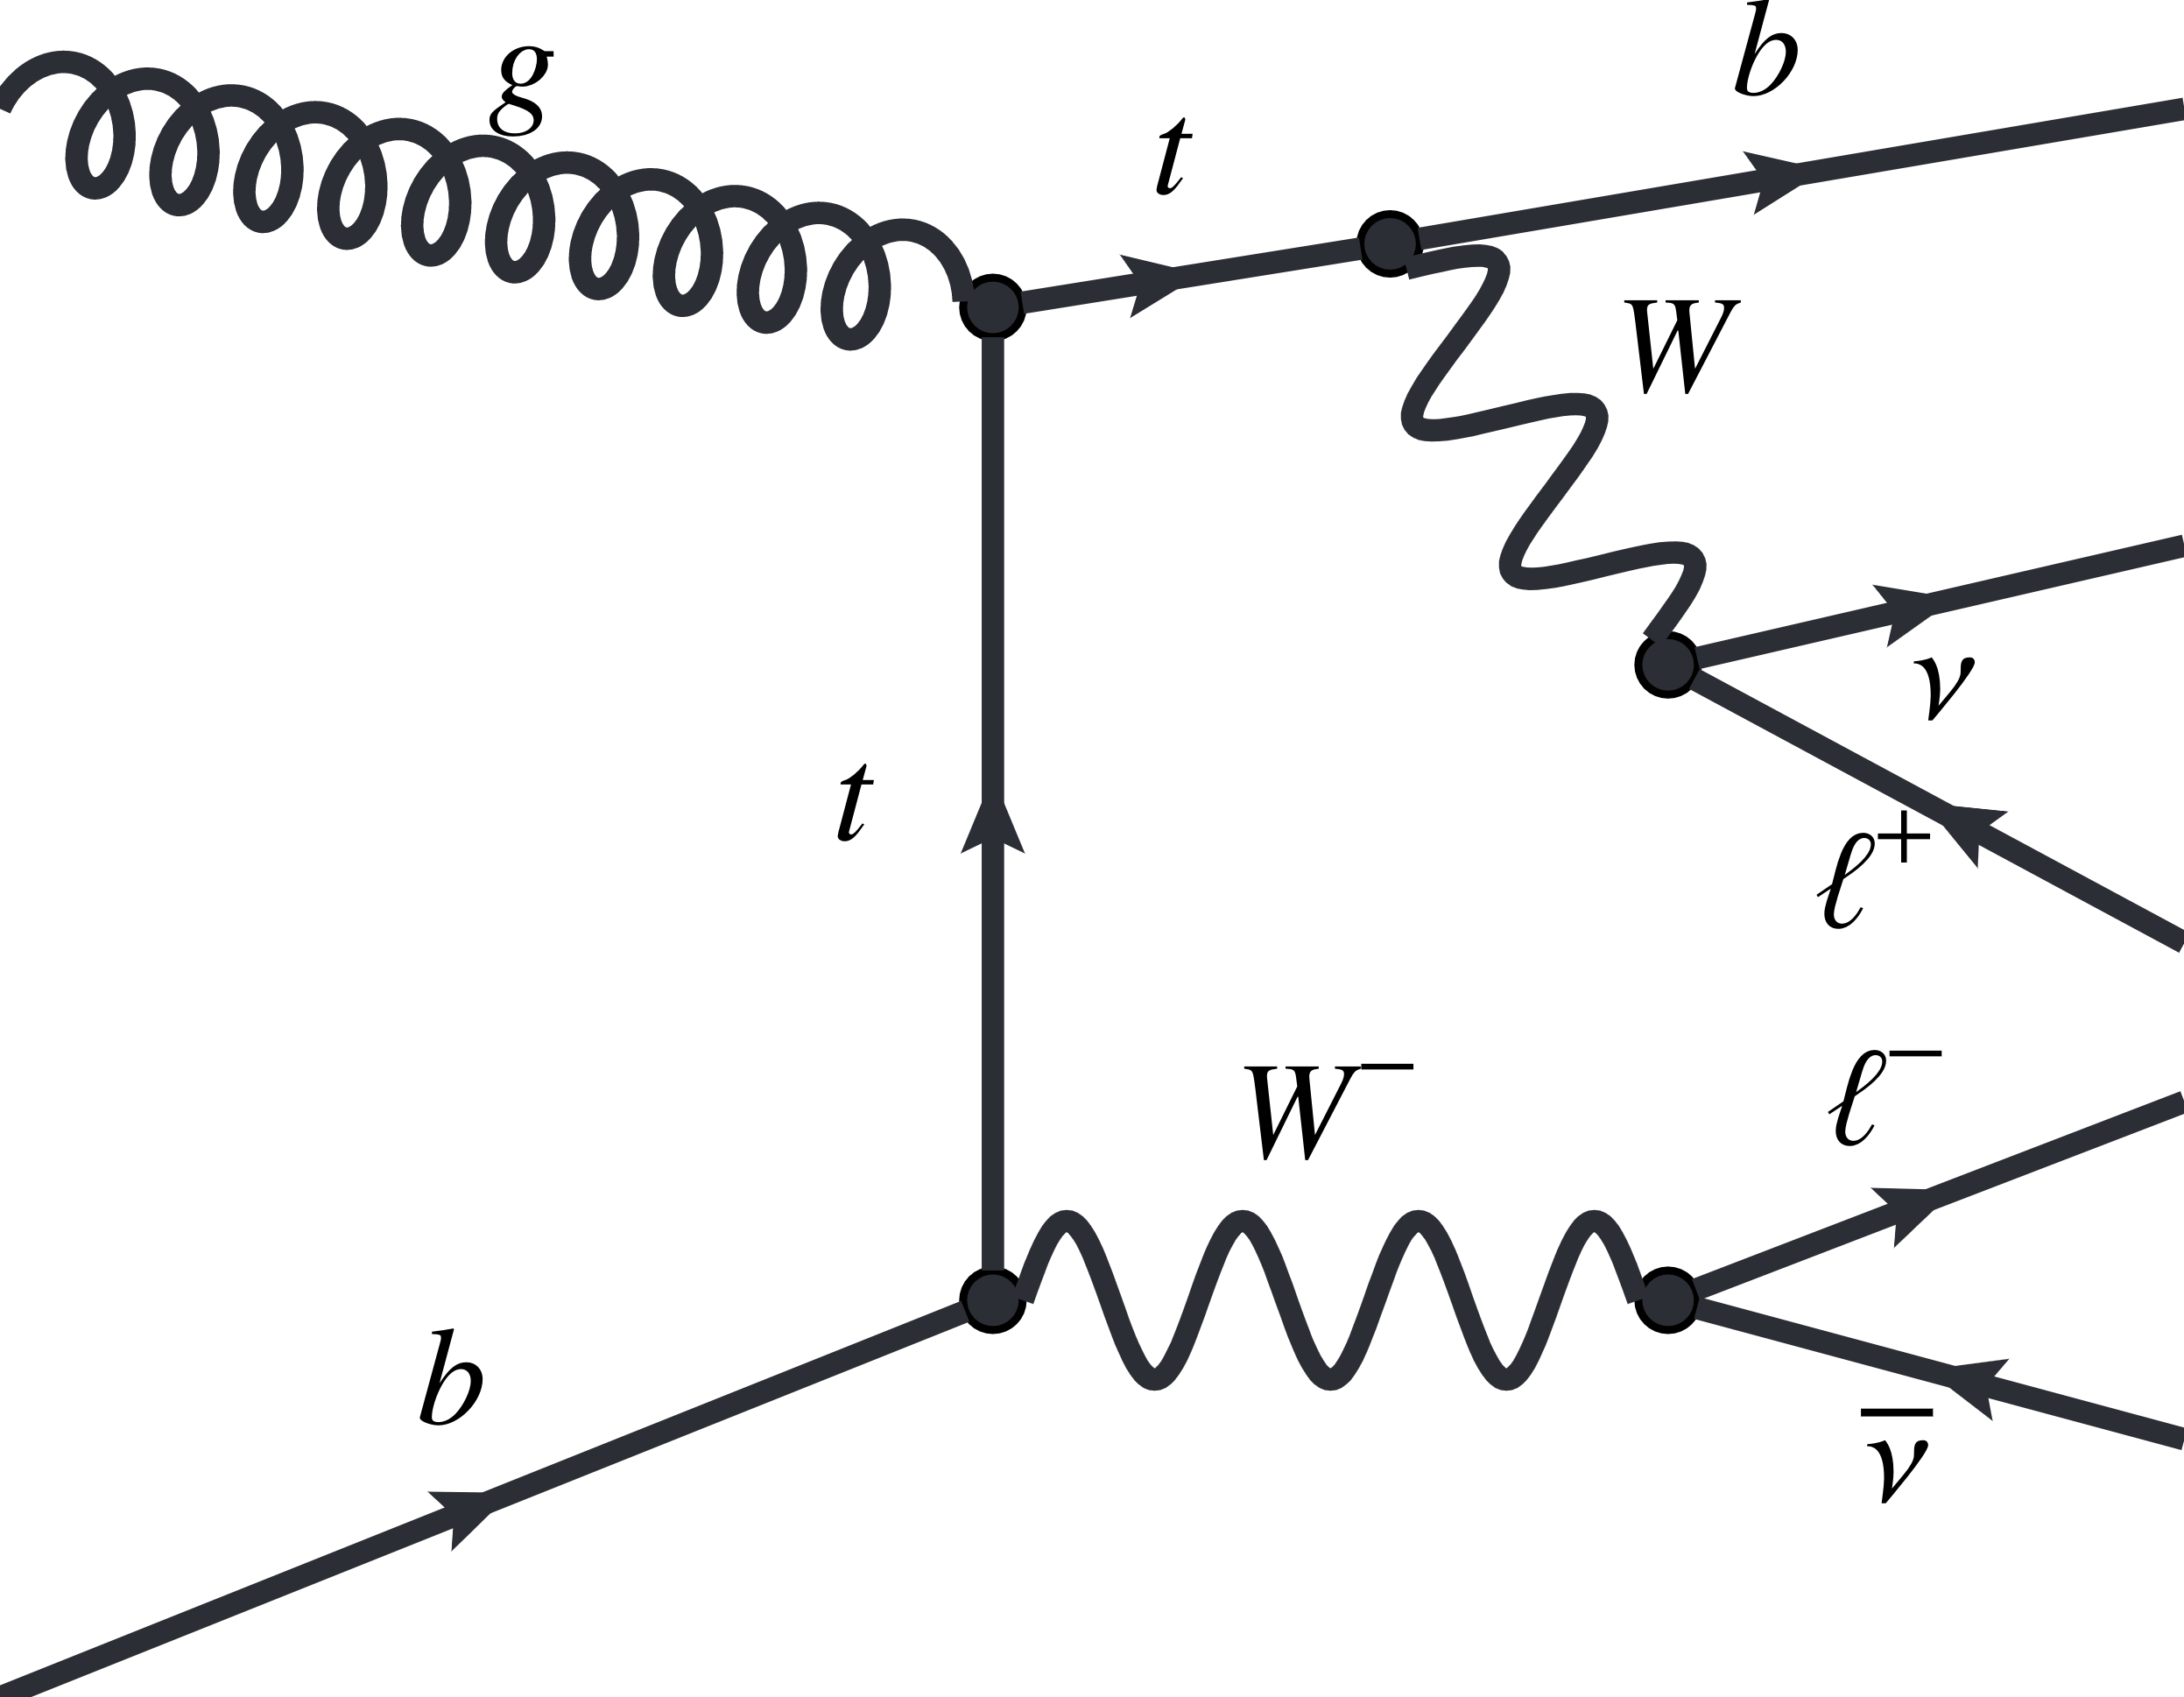
\includegraphics[width = 0.8\textwidth]{tw.png}
        \end{figure}
        \end{column}
        \begin{column}{0.5\textwidth}
        \begin{figure}
            \centering
            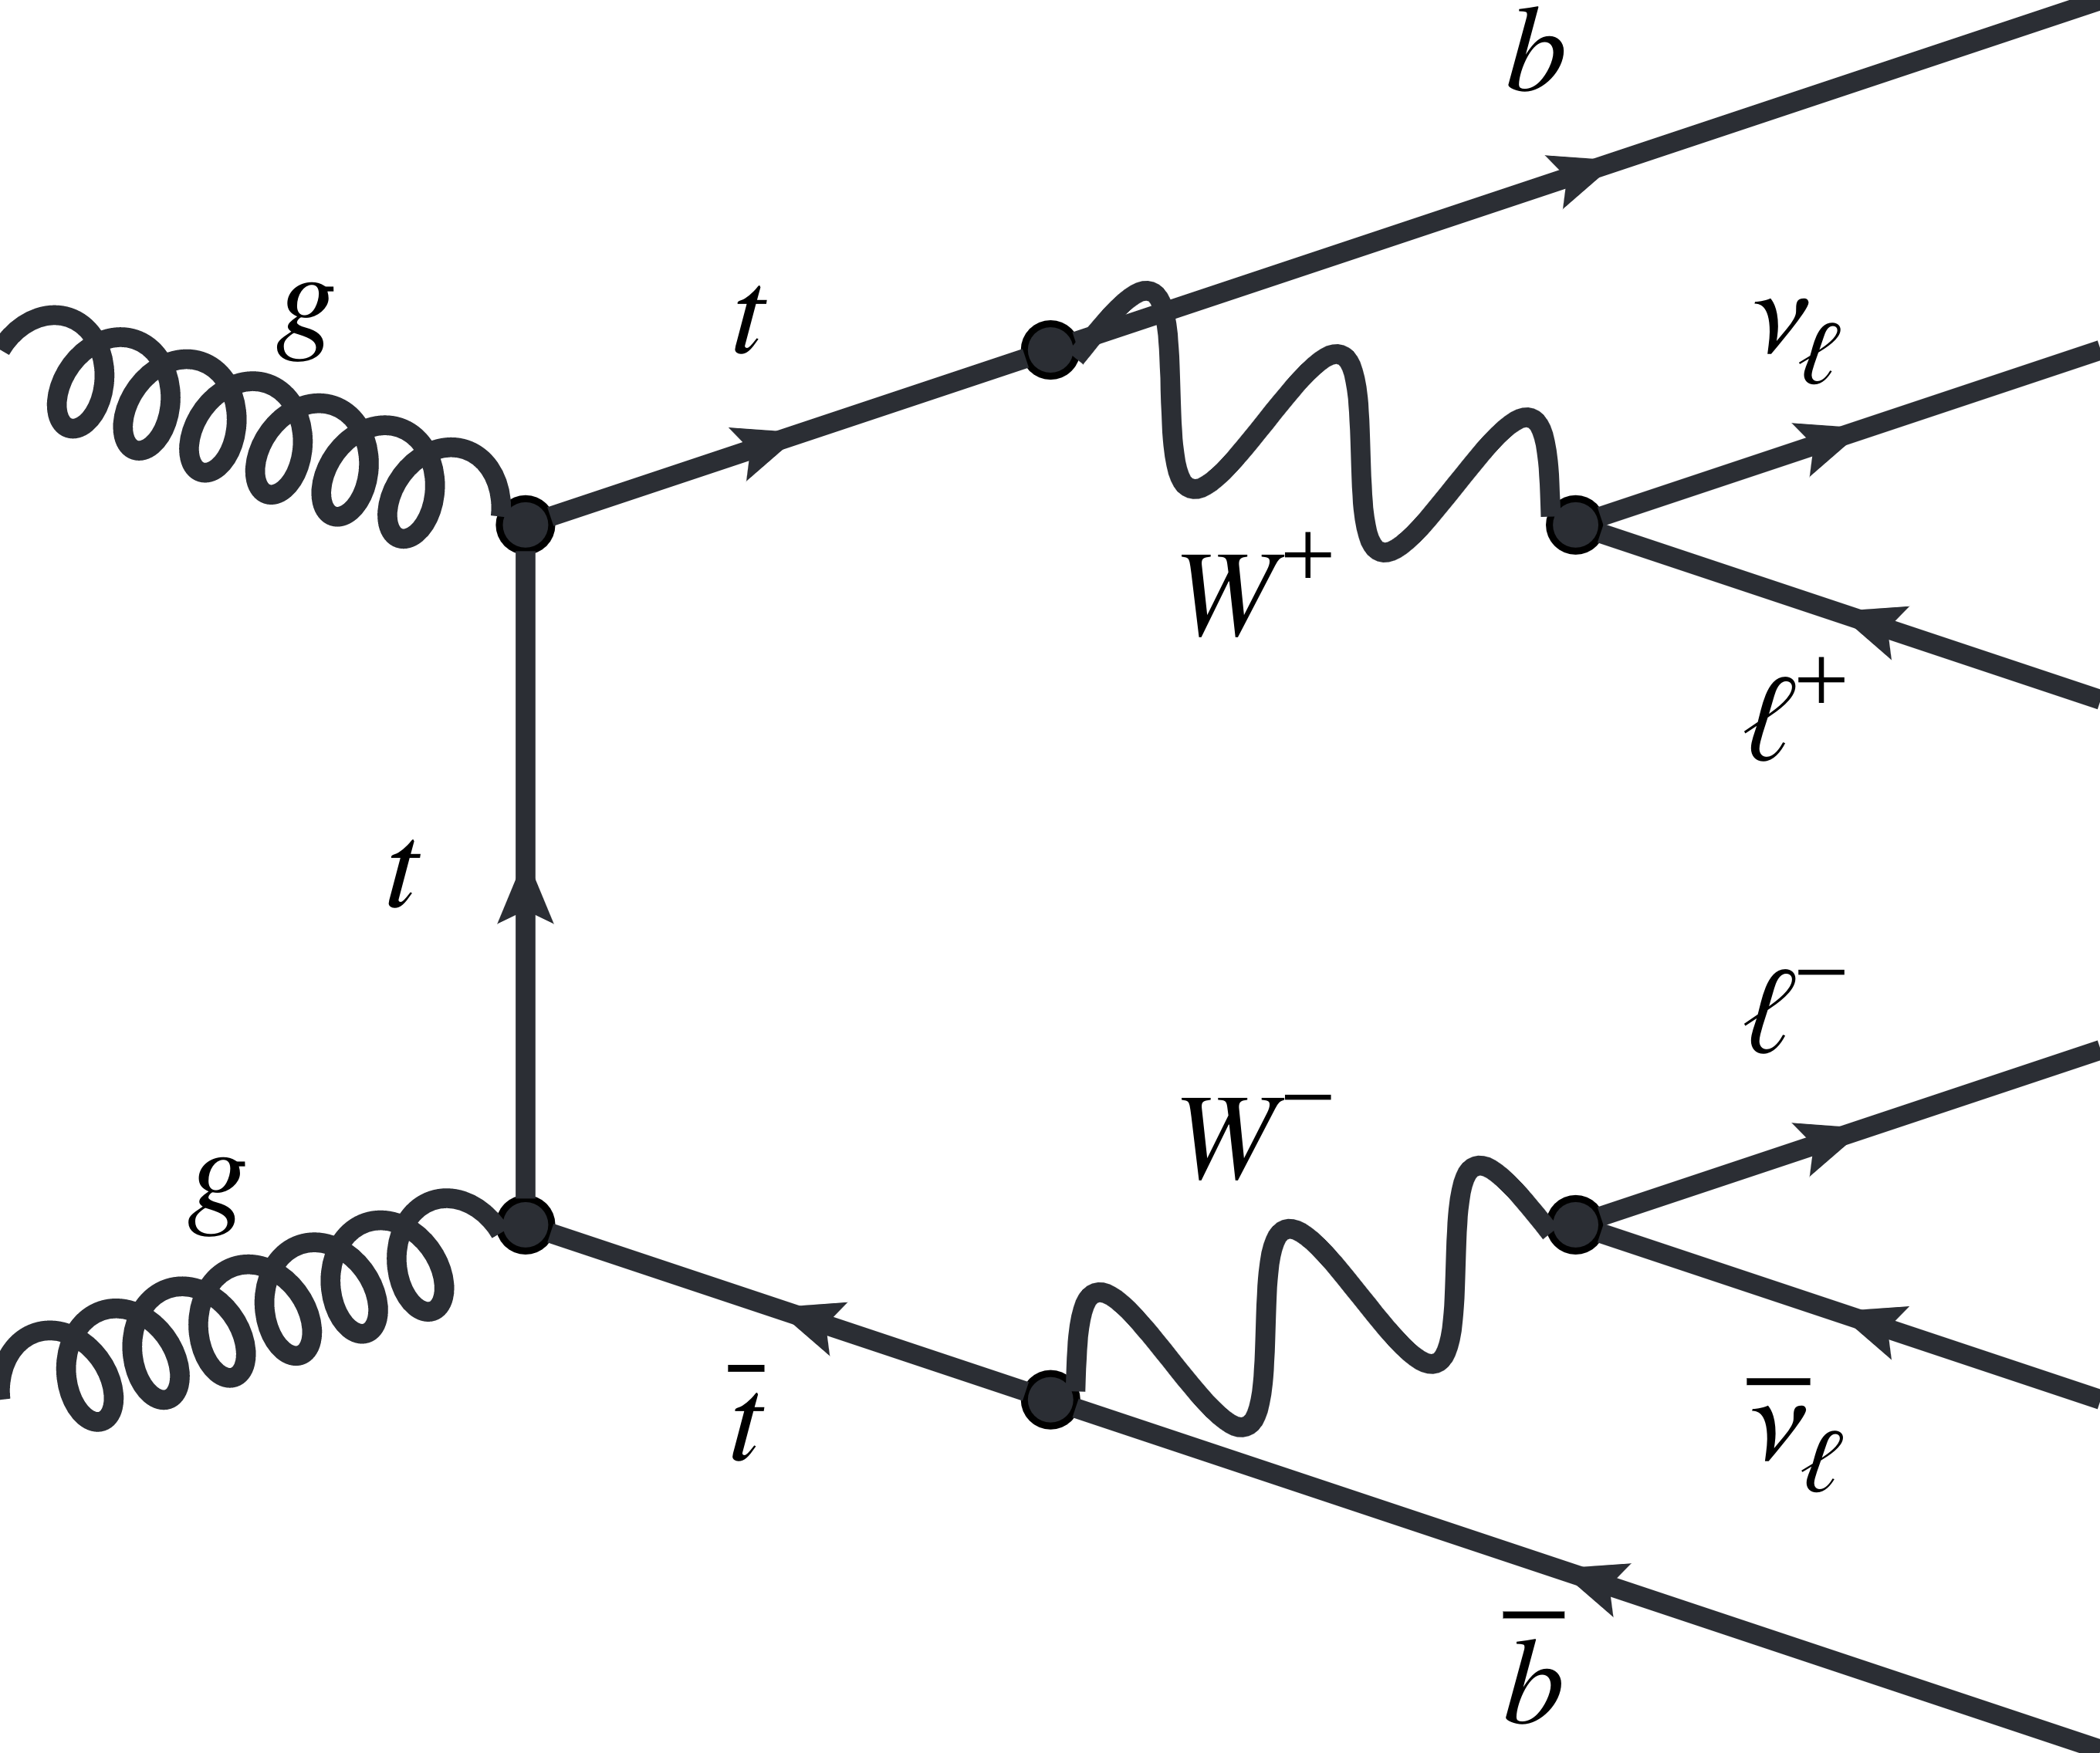
\includegraphics[width = 0.8\textwidth]{tt.png}
        \end{figure}
    \end{column}
\end{columns}
\begin{itemize}
    \item Problem: Cross-sections of $\Ptop\PW$ about 10 times smaller than $\Ptop\APtop$
    \item Interference in NLO order
    \item Instead of applying cut $\longrightarrow$ Neural networks
\end{itemize}
\end{frame}

\section{NN}

\begin{frame}{Setup of the classifier}
\begin{block}{Hyper-parameter scan results}
\begin{itemize}
\item Input: \num{14} variables motivated by a BDT variable scan.
\item Hidden layers: \num{6} \ELU layers $\times$ \num{128} nodes each
\item Output layer: \num{1} \SIGMOID node
\item Optimisation: SGD, \textcolor{red}{learning rate $=0.06$}, momentum $=0.3$, no nesterov, no decay
\item Duration: 600 epochs
\end{itemize}
\end{block}
\end{frame}

\begin{frame}{Simple network results}
\vspace{-2mm}
\begin{figure}[htbp]
    \centering
    \begin{subfigure}[b]{0.4\textwidth}
        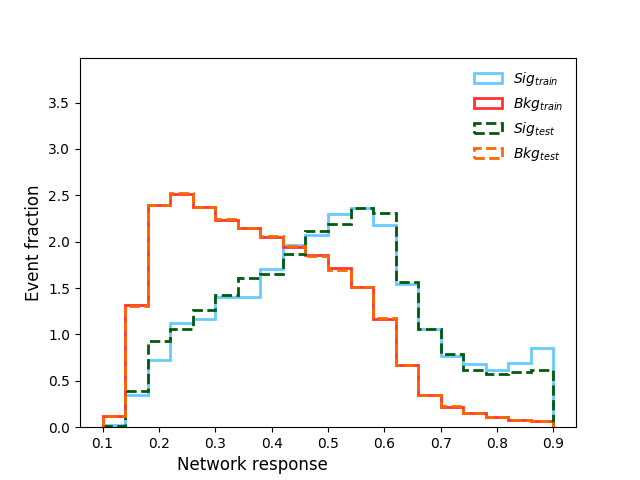
\includegraphics[width=\textwidth]{standard_separation}
        \caption{Separation}
        \label{fig:simple:final:sepa}
    \end{subfigure}
\quad
%    \begin{subfigure}[b]{0.4\textwidth}
%        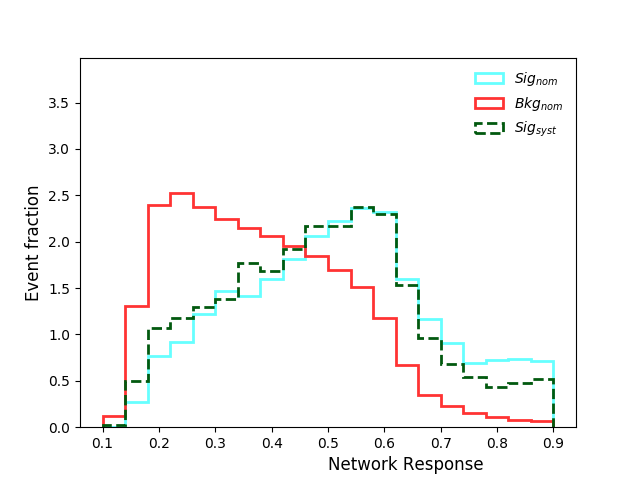
\includegraphics[width=\textwidth]{standard_syst}
%        \caption{Systematics}
%        \label{fig:simple:final:syst}
%    \end{subfigure}

    \begin{subfigure}[b]{0.4\textwidth}
		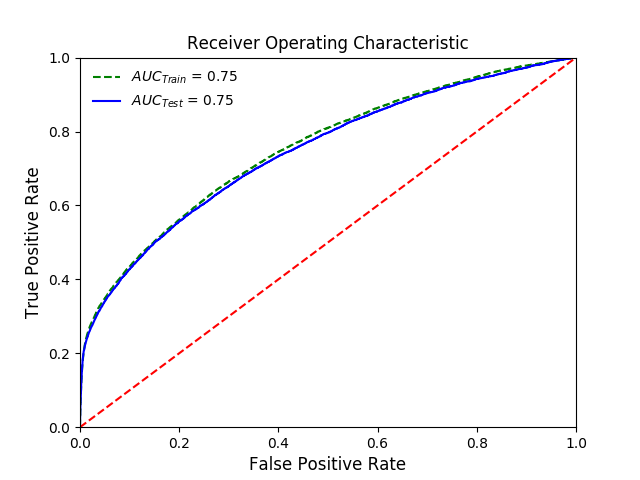
\includegraphics[width=\textwidth]{standard_ROC}
		\caption{ROC curve}
		\label{fig:simple:final:roc}
	\end{subfigure}
\quad
	\begin{subfigure}[b]{0.4\textwidth}
		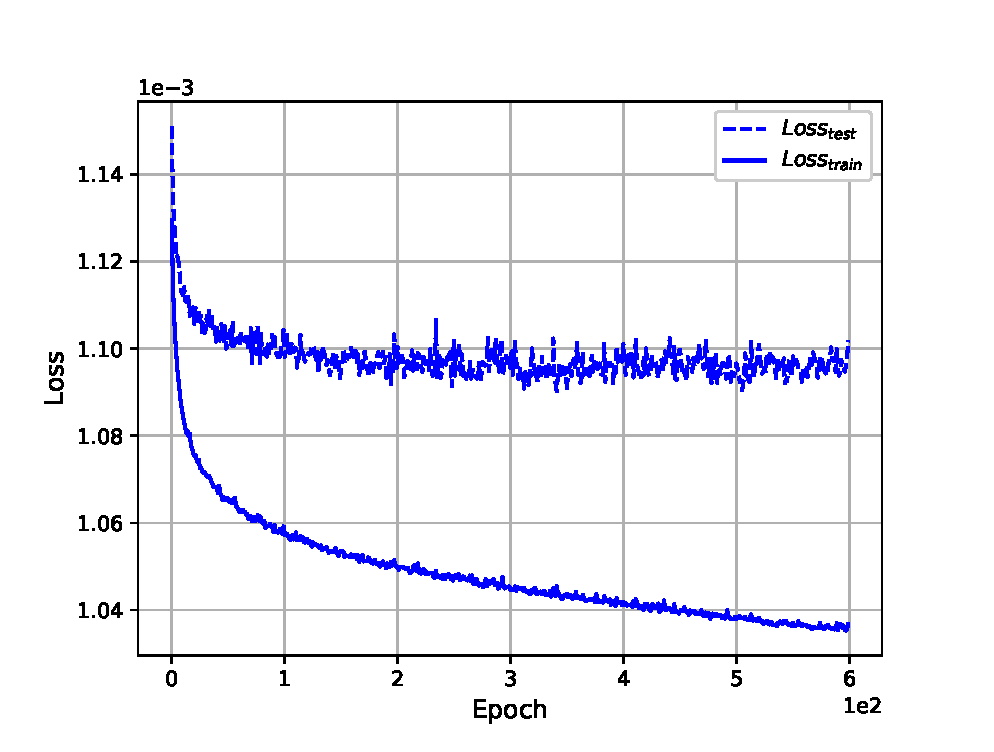
\includegraphics[width=\textwidth]{standard_losses}
		\caption{Losses}
		\label{fig:simple:final:loss}
	\end{subfigure}
\end{figure}
\end{frame}

\section{ANN}

\begin{frame}{Adversarial Neural Networks}
    \begin{itemize}
        %\item Originally introduced as Generative adversarial %neural networks to overcome weaknesses of generative %networks \cite{2014arXiv1406.2661G}
        \item Neural networks have no info on systematic uncertainties 
        \vspace{0.2cm}
        \item Introduction of a second, adversarial network classifying between nominal and systematic
        \vspace{0.2cm}
        \item Combined loss function $\mathcal{L}_{adversarial}\left( \theta_f, \theta_t \right) = \mathcal{L}(\theta_f) - \lambda \mathcal{L}(\theta_f, \theta_r)$
        \vspace{0.2cm}
        \item Network 1: signal/background separation
        \vspace{0.2cm}
        \item Network 2: nominal/systematic separation
        \vspace{0.2cm}
        \item Expectation: network 1 succeeds, network 2 fails
    \end{itemize}
\end{frame}

\begin{frame}{Setup of the ANN}
    \begin{figure}
        \centering
        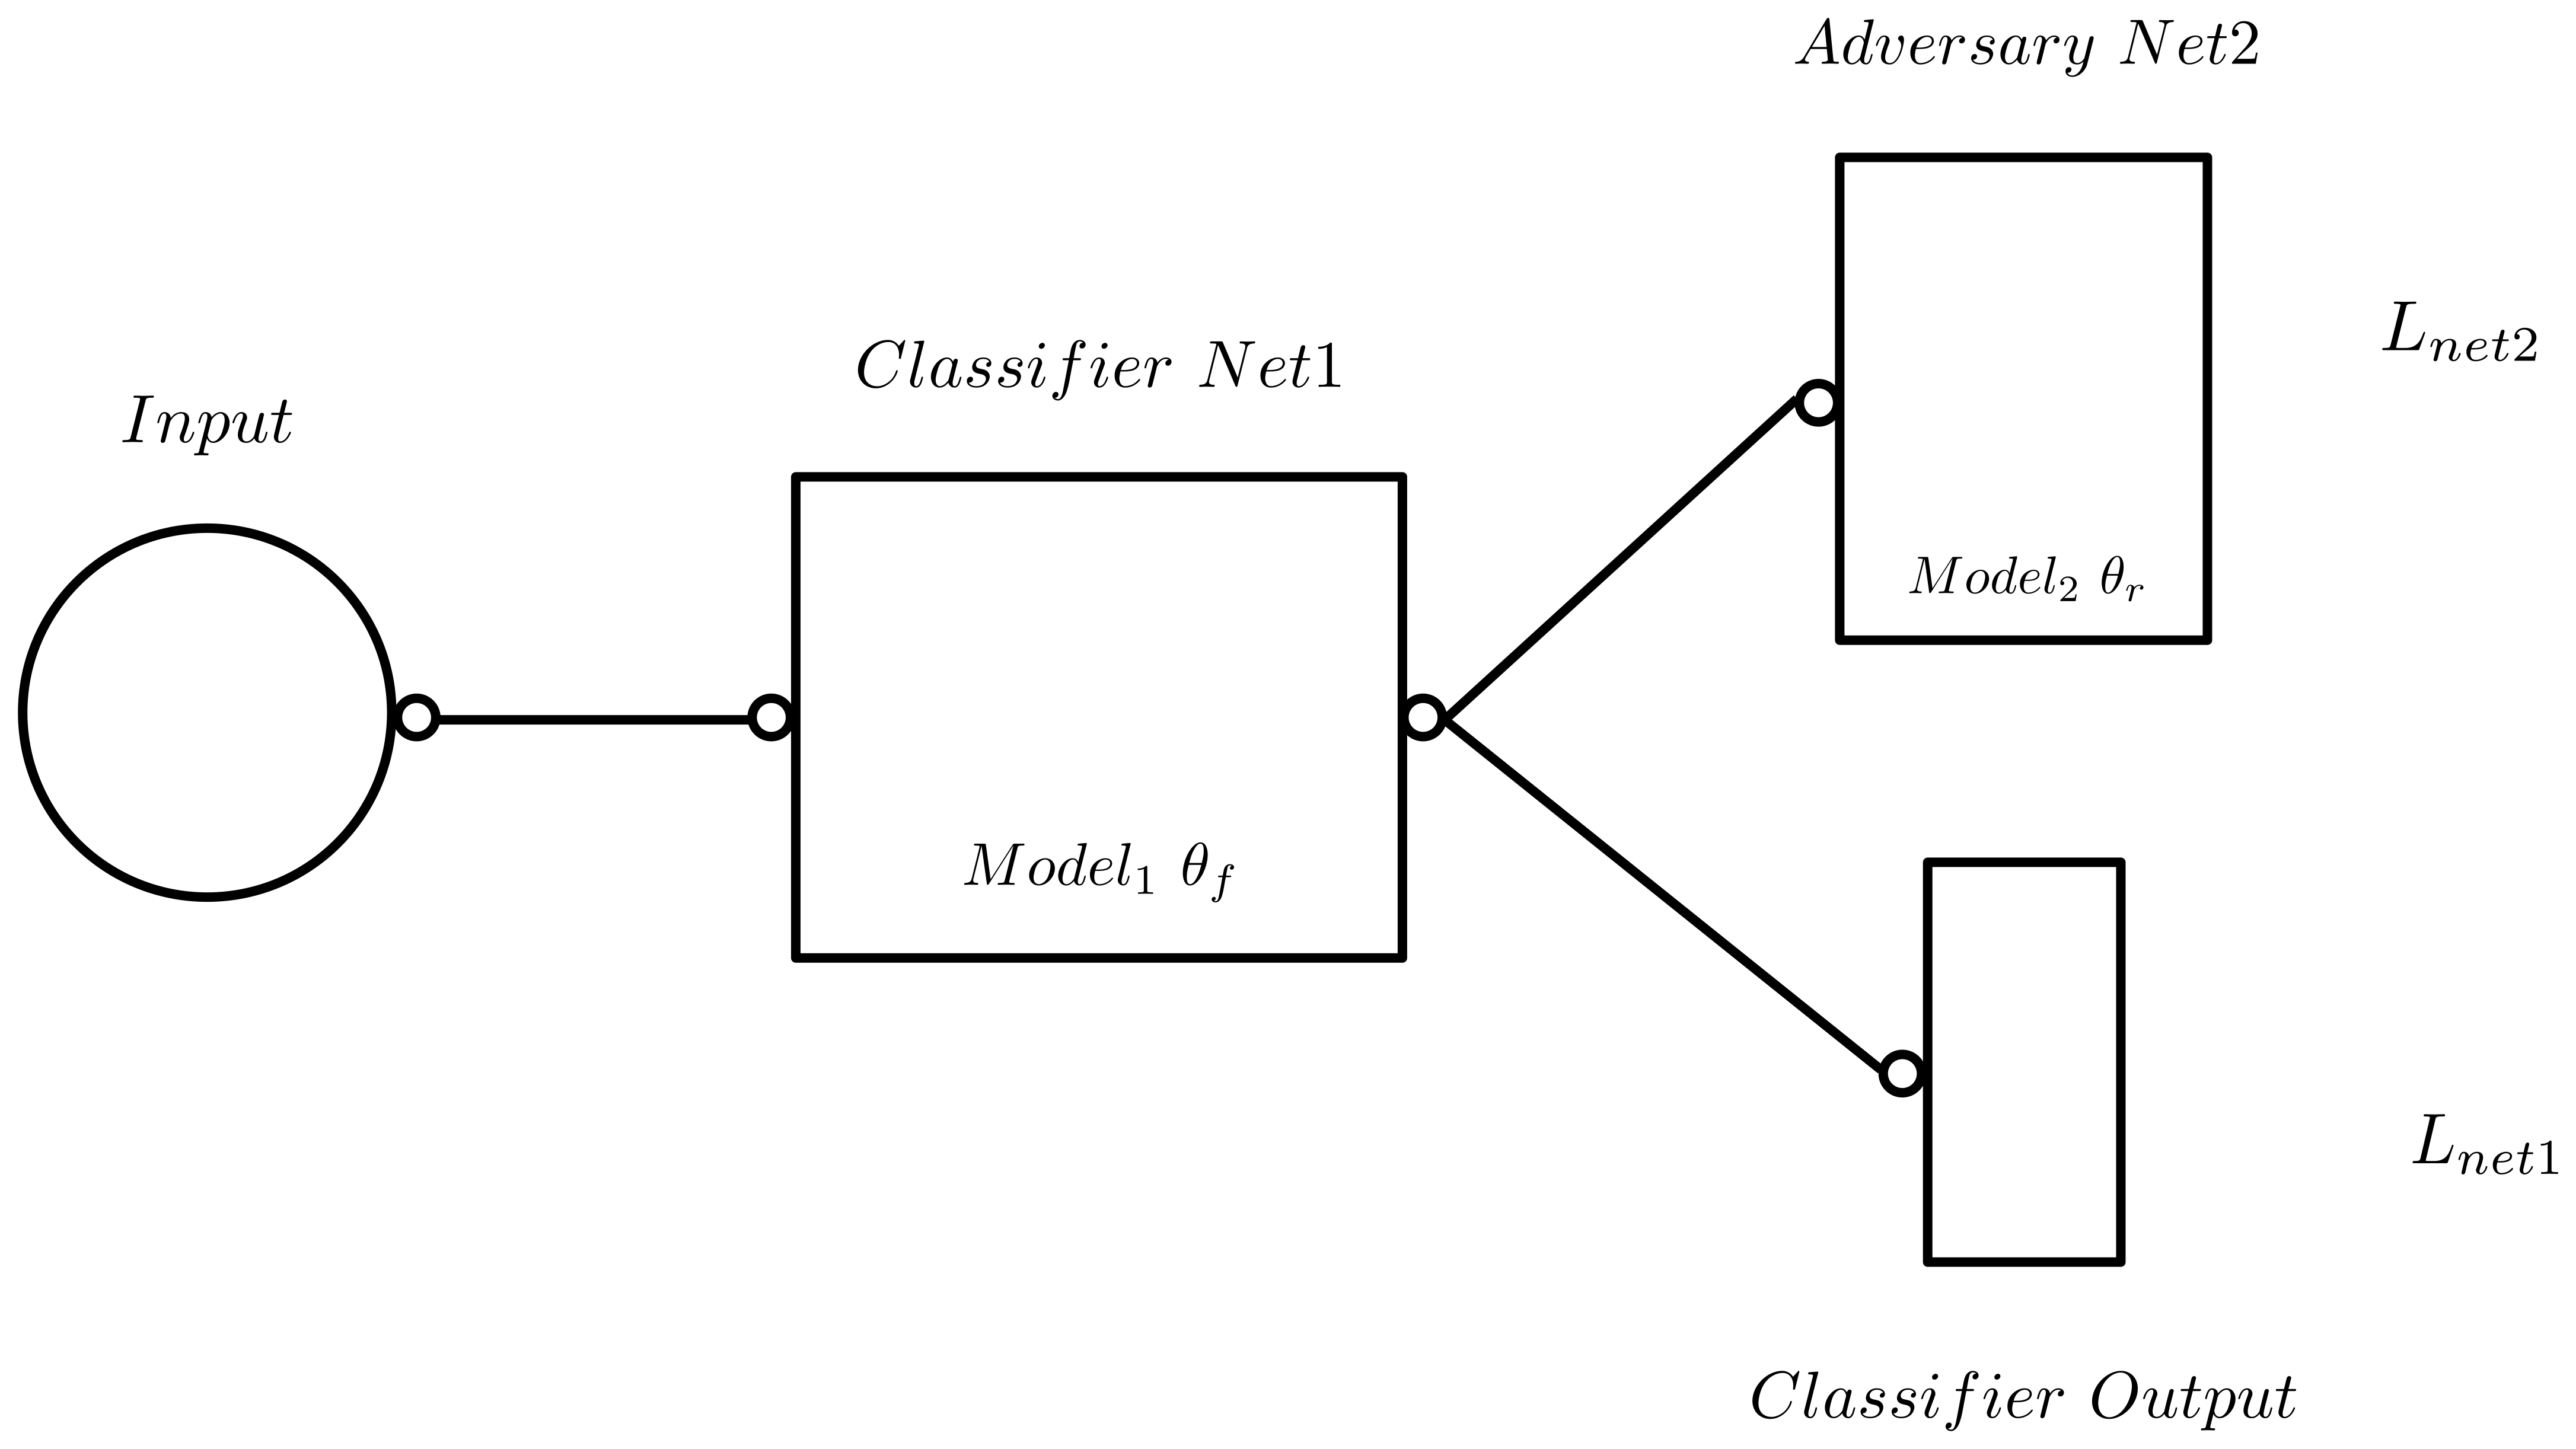
\includegraphics[width=\textwidth]{ANN_sketch.png}
        \label{fig:my_label}
    \end{figure}
\end{frame}

\begin{frame}{ANN}
\begin{table}[]
\begin{tabular}{|l|l|l|}
\hline
                      & Discriminator & Adversary \\ \hline
\ttbar &         0      &     1      \\ \hline
\tW DR &         1     &      1    \\ \hline
\tW DS &         1     &      0    \\ \hline
\end{tabular}
\end{table}
\end{frame}

\begin{frame}{ANN setup}
\begin{block}{Discriminator setup}
\begin{itemize}
\item Input: \num{14} variables motivated by a BDT variable scan.
\item Hidden layers: \num{6} \ELU layers $\times$ \num{128} nodes each
\item Output layer: \num{1} \SIGMOID node
\item Optimisation: SGD, \textcolor{red}{learning rate $=0.01$}, momentum $=0.3$, no nesterov, no decay
\end{itemize}
\end{block}
\begin{block}{Adversary setup}
\begin{itemize}
\item Input: \num{14} variables motivated by a BDT variable scan.
\item Hidden layers: \num{6} \ELU layers $\times$ \num{128} nodes each
\item Output layer: \num{1} \SIGMOID node
\item Optimisation: SGD, \textcolor{red}{learning rate $=0.01$}, momentum $=0.3$, no nesterov, no decay
\end{itemize}
\end{block}
\end{frame}

\begin{frame}{ANN results}
\begin{figure}[htbp]
    \centering
    \begin{subfigure}[b]{0.4\textwidth}
		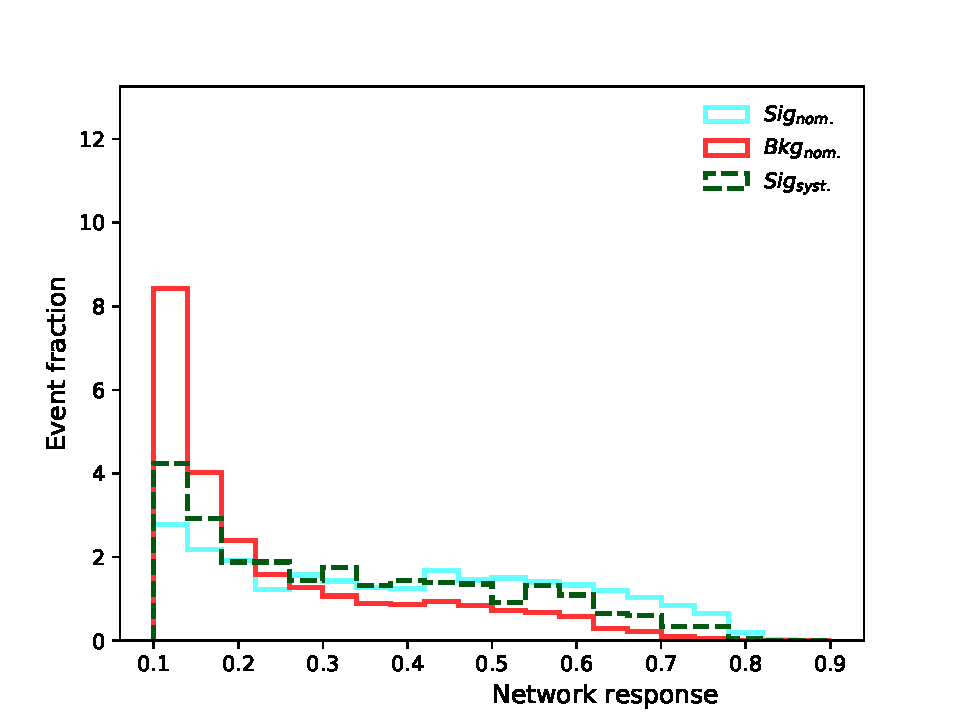
\includegraphics[width=\textwidth]{app2_syst.pdf}
		\caption{Separation}
		\label{fig:simple:final:roc}
	\end{subfigure}
\quad
	\begin{subfigure}[b]{0.4\textwidth}
		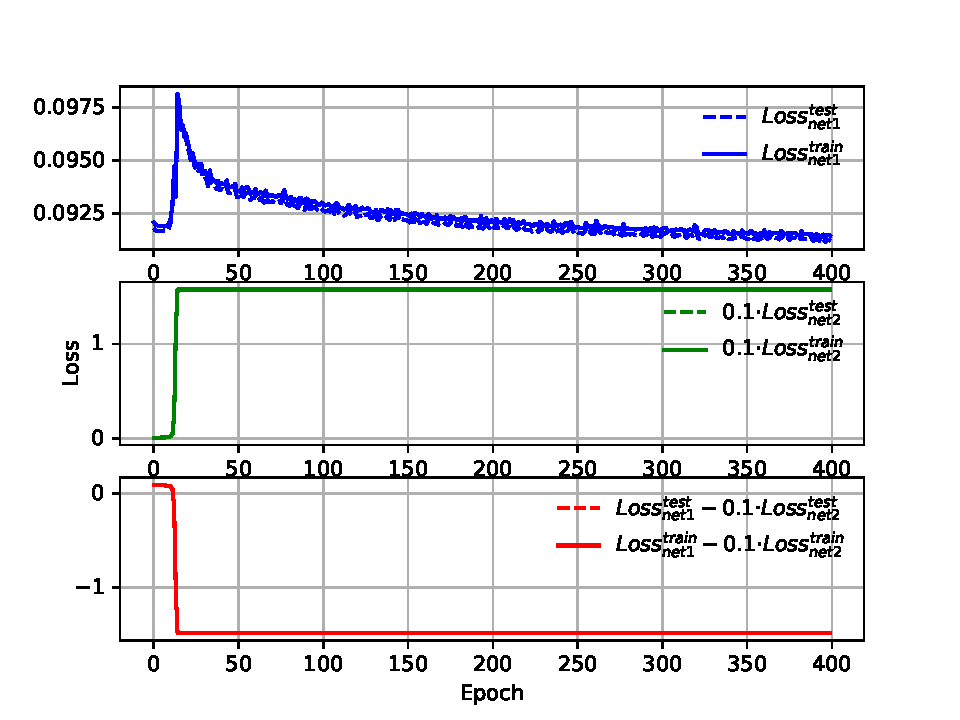
\includegraphics[width=\textwidth]{app2_losses2.pdf}
		\caption{Losses}
		\label{fig:simple:final:loss}
	\end{subfigure}
\end{figure}
\begin{itemize}
\item The separation is visibly bad.
\item The agreement between nominal and systematics has barely improved
\item Losses show bad behaviour
\end{itemize}
\end{frame}


\section{Background Labeling}

\begin{frame}{Improvement plans}
\begin{block}{Assumption}
    Labelling \ttbar as a nominal sample results in a strong bias
\end{block}
\begin{block}{Possible solution}
    \begin{itemize}
        \item Randomly label \ttbar events as either nominal or systematic
        \item Add additional weighting to the \ttbar sample for the adversarial network only
        \item Exclude the \ttbar sample for the adversarial training completely
    \end{itemize}
\end{block}
\end{frame}

\begin{frame}{Applied fixes}
\begin{block}{Re-labelling}
\begin{table}[]
\begin{tabular}{|l|l|l|}
\hline
                      & Discriminator & Adversary \\ \hline
\ttbar &         0      &     1/0 (50 \% mix)     \\ \hline
\tW DR &         1     &      1    \\ \hline
\tW DS &         1     &      0    \\ \hline
\end{tabular}
\end{table}
\end{block}
\begin{block}{Weighting \ttbar for the adversary}
\begin{itemize}
\item Applying an additional weight to the \ttbar events for the adversarial training only
\item Varied the weights between \num{0.0} and \num{1.0}
\end{itemize}
\end{block}
\end{frame}


\begin{frame}{ttbar weights for the adversarial training}
    \begin{figure}[htbp]
    \caption{Weight = 0}
    \centering
    \begin{subfigure}[b]{0.47\textwidth}
        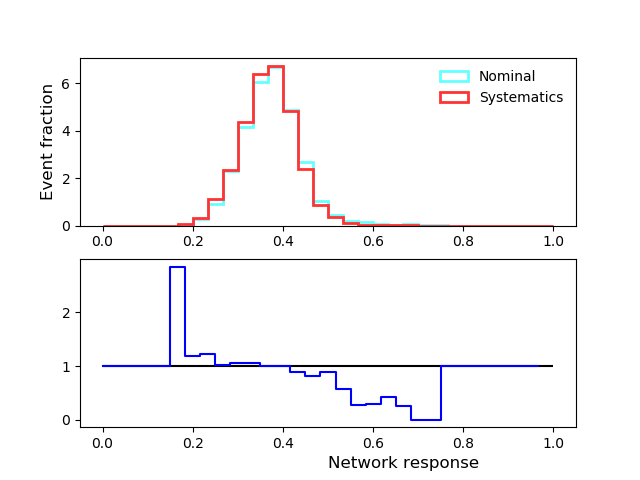
\includegraphics[width=0.8\textwidth]{separation_adversaryweight0.png}
        \label{fig:simple:final:sepa}
    \end{subfigure}
\quad
    \begin{subfigure}[b]{0.47\textwidth}
        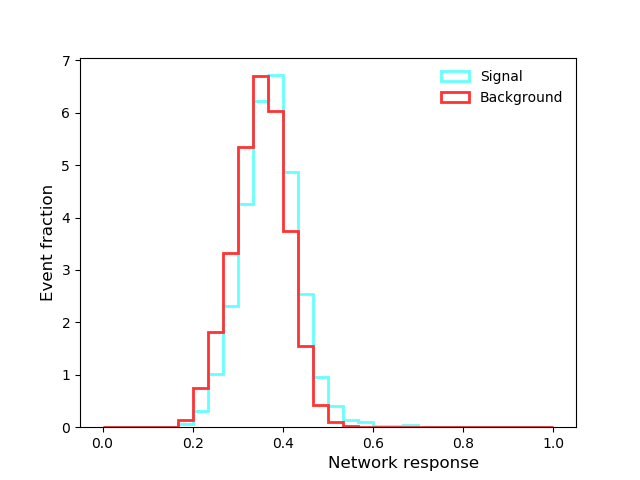
\includegraphics[width=0.8\textwidth]{separation_discriminatorweight0.png}
        \label{fig:simple:final:syst}
    \end{subfigure}
    \end{figure}
    \vspace{-0.7cm}
    \begin{figure}[htbp]
    \caption{Weight = 1}
    \centering
    \begin{subfigure}[b]{0.47\textwidth}
        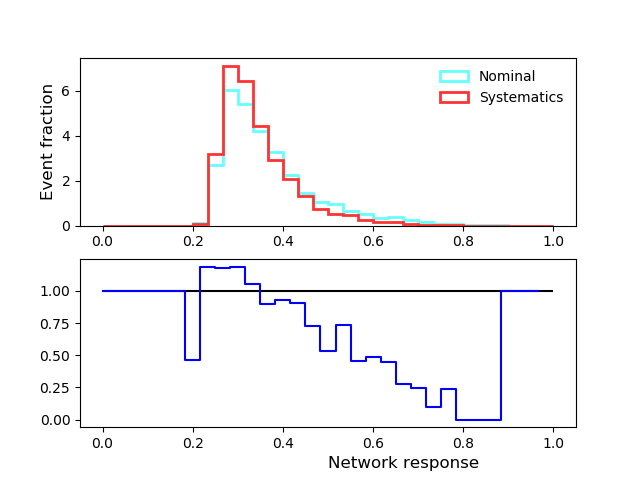
\includegraphics[width=0.8\textwidth]{separation_adversaryweight1.png}
        \label{fig:simple:final:sepa}
    \end{subfigure}
\quad
    \begin{subfigure}[b]{0.47\textwidth}
        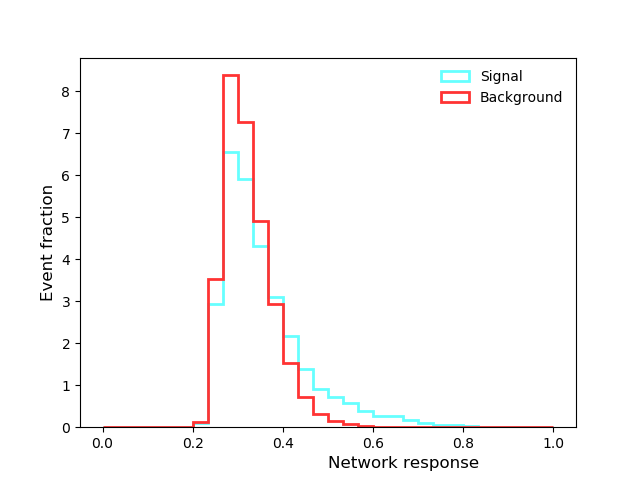
\includegraphics[width=0.8\textwidth]{separation_discriminatorweight1.png}
        \label{fig:simple:final:syst}
    \end{subfigure}
    \end{figure}
\end{frame}



\begin{frame}{ttbar weights for the adversarial training}
    \begin{figure}[htbp]
    \caption{Weight = 0}
    \centering
    \begin{subfigure}[b]{0.47\textwidth}
        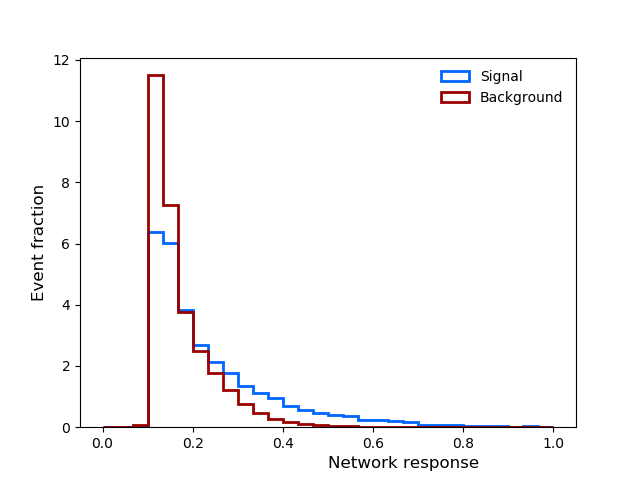
\includegraphics[width=0.8\textwidth]{discriminator_50per.png}
        \label{fig:simple:final:sepa}
    \end{subfigure}
\quad
    \begin{subfigure}[b]{0.47\textwidth}
        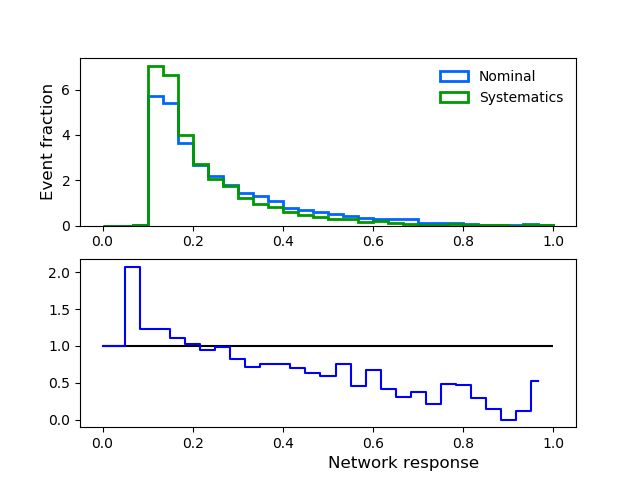
\includegraphics[width=0.8\textwidth]{adversary_50per.png}
        \label{fig:simple:final:syst}
    \end{subfigure}
    \end{figure}
    \vspace{-0.7cm}
    \begin{figure}[htbp]
    \caption{Weight = 1}
    \centering
    \begin{subfigure}[b]{0.47\textwidth}
        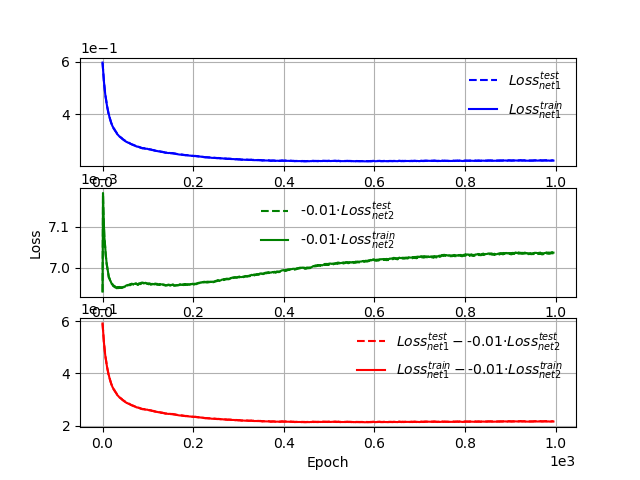
\includegraphics[width=0.8\textwidth]{losses_50per.png}
        \label{fig:simple:final:sepa}
    \end{subfigure}
\quad
    \begin{subfigure}[b]{0.47\textwidth}
        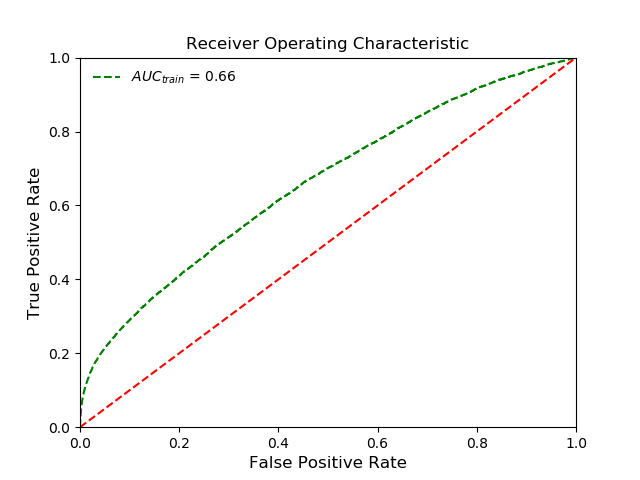
\includegraphics[width=0.8\textwidth]{roc_50per.png}
        \label{fig:simple:final:syst}
    \end{subfigure}
    \end{figure}
\end{frame}


\begin{frame}{Conclusions}
\begin{block}{Improvements and insights}
\begin{itemize}
\item sdfw
\end{itemize}
\end{block}
\begin{block}{Weighting \ttbar for the adversary}
\begin{itemize}
\item Applying an additional weight to the \ttbar events for the adversarial training only
\item Varied the weights between \num{0.0} and \num{1.0}
\end{itemize}
\end{block}
\end{frame}

\section{Conclusions}





\end{document}